\chapter{Generative Models}
% \chapter{ Autoencoders }
% Authors: Bixing Yan (by783), Chengze Zuo (cz1565) , Yavuz Sunor (ys3226) Apr 14, 2019.
% Editor: Benjamin Ahlbrand
\section{ Autoencoders }

Autoencoders fall under a class of unsupervised generative models. Generative models are unsupervised learning algorithms aiming at learning the true data distributions of the training set so as to generate new data points with some variations. They are widely used in image processing for super resolution / upscaling algorithms, additionally in inpainting and image captioning, to name but a few applications.

Autoencoders exploit information bottlenecking in order to learn an efficient encoding of the latent space of the data distribution. With the neural network architecutre splits into an encoder and decoder. The aim of an autoencoder is to restore its input data at the output. Traditionally, autoencoders have been used for dimensionality reduction; while recently, this concept is more widely used for learning the generative model of data.

The schematic illustration is shown as below:

\begin{figure}[htb]
    \centering
    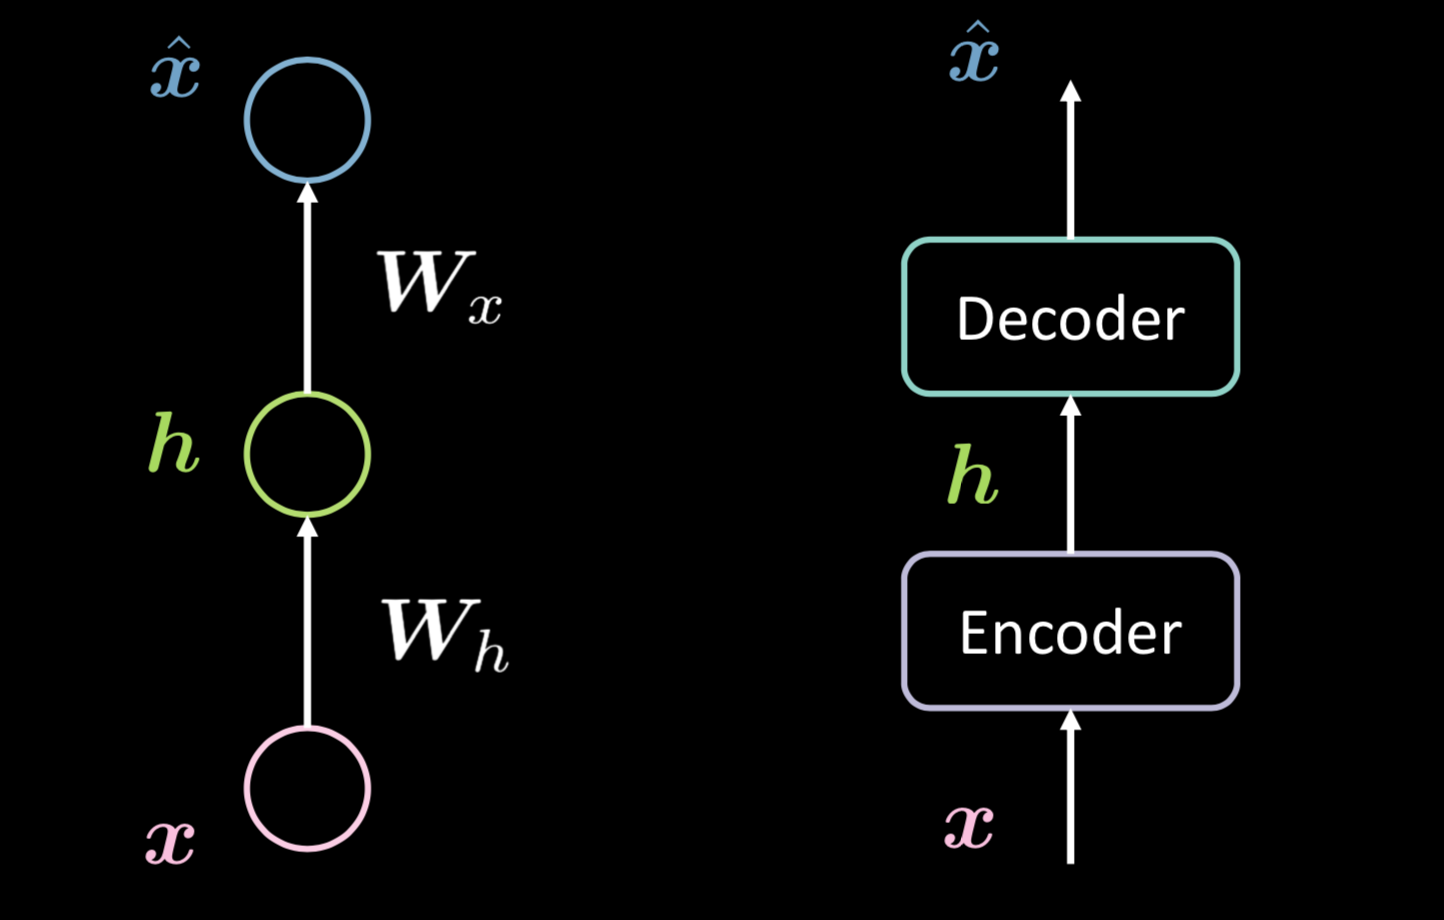
\includegraphics[width=0.6\textwidth]{figs/Schematic_Illustration_of_Autoencoder.png}
    \caption{Schematic Illustration of Autoencoder}
    \label{fig:Schematic_Illustration_of_Autoencoder}
\end{figure}

We observe in the above figure, typically, an autoencoder consists of two modules: the encoder and the decoder. The encoder will map the input data to a hidden space or latent code ($f_h: x\rightarrow h$), afterwards, the decoder will project the data from the target space back to the original input space ($f_x: h\rightarrow \hat{x}$).

The performance of an autoencoder is evaluated by how accurately the decoder can reconstruct the data after it is projected to a latent space (the code) by the encoder. Thus, the loss of an autoencoder is inversely correlated with the similarity between the input $x$ and the output $\hat{x}$ (or often referred to as the reconstruction loss). 
$$ L=\frac{1}{m}\sum_{j=1}^m l(x^j,\hat{x}^j) $$
For example, for the binary output, the entropy loss is usually used as the evaluation metric:
$$ l(x,\hat{x}) = -\sum_{i=1}^n[x_i\log(\hat{x}_i) + (1-x_i)\log(1-\hat{x}_i) ]$$
Additionally, for the real value output, the performance of an autoencoder is usually evaluated with the euclidean distance measure:
$$ l(x,\hat{x}) = \frac{1}{2} \| x-\hat{x} \|^2 $$
By optimizing in order to minimize the loss, we can train the autoencoder.

Depending on the dimension of the coded space (latent space or hidden layer), the autoencoder can be described as under-complete or over-complete, as the figure shown below:

\begin{figure}[htb]
    \centering
    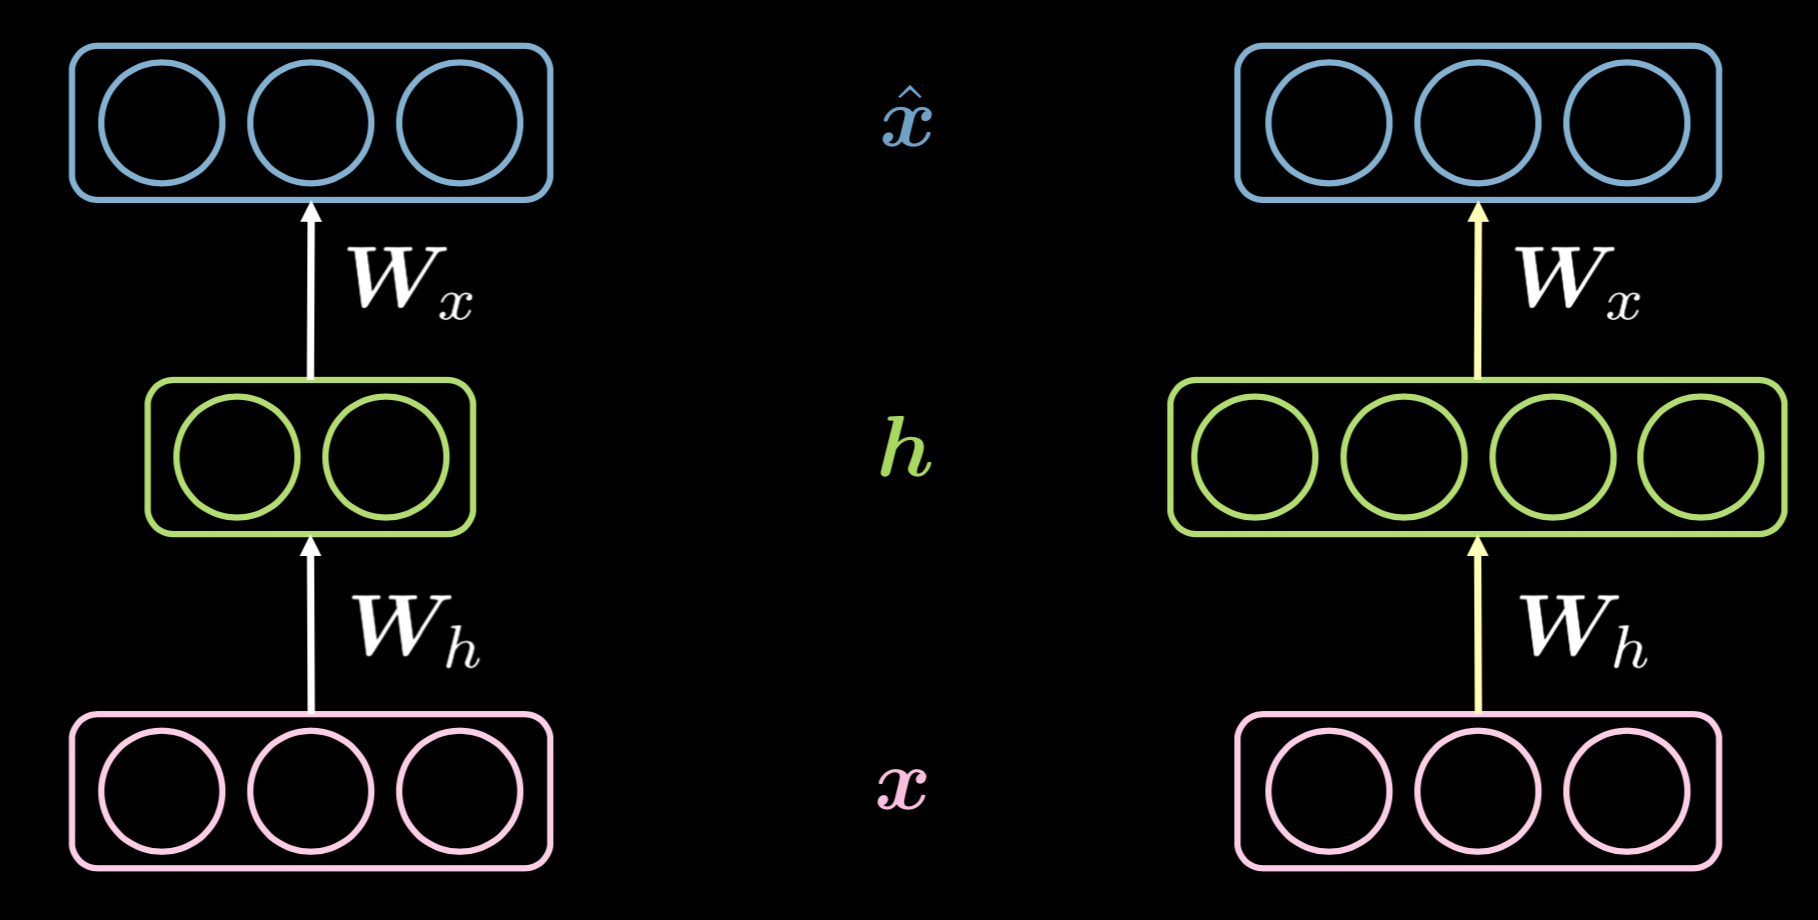
\includegraphics[width=0.6\textwidth]{figs/Under_(over)_complete_Autoencoder.png}
    \caption{Under-complete (left) and over-complete (right) Autoencoder}
    \label{fig:Under_(over)_complete_Autoencoder}
\end{figure}

In accordance with the names, the size of the hidden layer of an under-complete autoencoder will be smaller than the input size; while that of an over-complete one will be large than the input size. The under-complete auto encoder is usually applied to perform dimension reduction, while the over-complete autoencoder is utilized to learn features.

More specific, for an under-complete autoencoder, the dimension of the hidden layer would be smaller than the instrinsic dimension of data manifold (The point here is to learn the feature. If you have same number of neurons, you can just simply copy). So this type of autoencoder will encode features that are important for reconstructing (usually will introduce constraints from previous layers). In other words, by training an under-complete representation, we force the autoencoder to learn the most salient features of the training data. That's why, an under-complete autoencoder will perform well when reconstructing samples similar to training samples, but bad with other types of inputs.  

As for over-complete autoencoders, more units in the hidden layer would not guarantee that the hidden units will extract meaningful structure, but most likely copy the input element by element. However, if we are interested in a linear classifier, more dimension allows the network to learn more/better features (higher dimension is better). So, for example, this particular class of autoencoders doesn't perform well with MNIST dataset which requires non-linearity to learn separable patterns. Two ways to deal with this problem and extract meaningful features are using denoising and contractive autoencoders.

\subsection{Denoising Autoencoder}

The input of denoising autoencoders is a partially corrupted input whilst training to recover the original undistorted input. The denoising autoencoder mainly focuses on robust representations of inputs and extracting features that are useful for representation of the input distribution.

As the description above, to train the autoencoder, we need to corrupt the data with noise ($x \rightarrow x'$). The distribution of the noise will be comparable to our observation in reality, so that the denoising autoencoder can robustly recover the real data.
One thing need to note here is, because the ideal output $\bar{x}$ are expected to be the clean data $x$ rather than the noised input $x'$, the loss is a function of $x$ and $\bar{x}$, i.e., $l(x,\bar{x})$ rather than $l(x',\bar{x})$.

A schematic illustration of the corruption and denoising process is shown below:

\begin{figure}[htb]
    \centering
    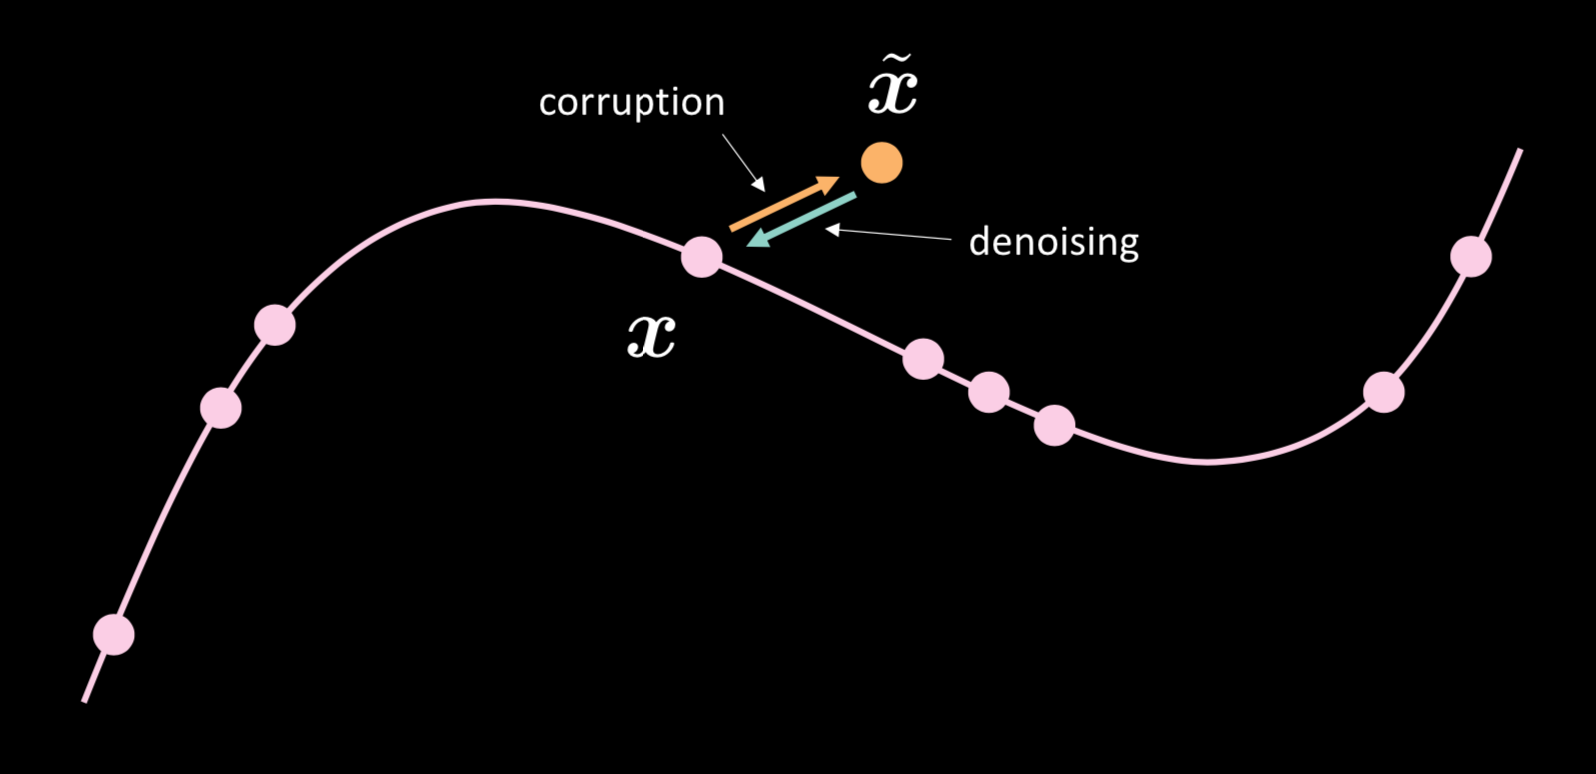
\includegraphics[width=0.6\textwidth]{figs/Corrpution_and_Denoising.png}
    \caption{Corruption and Denoising Process for Denoising Autoencoder}
    \label{fig:Corrpution_and_Denoising}
\end{figure}

\subsection{Contractive Autoencoder}

A contractive autoencoder makes this encoding less sensitive to small variations in its training dataset. This is achieved by adding an explicit regularizer to the objective function in order to to force the model to learn a function that is robust to slight variations of input values. The loss function includes a term that penalizes insensitivity to the reconstruction direction and a term that penalizes sensitivity to all directions:

$$l(x,\bar{x}) = l_{\text{reconstruction}} + \lambda \| \nabla_x h \|^2$$

A schematic illustration of this concept is shown below: 

\begin{figure}[H]
    \centering
    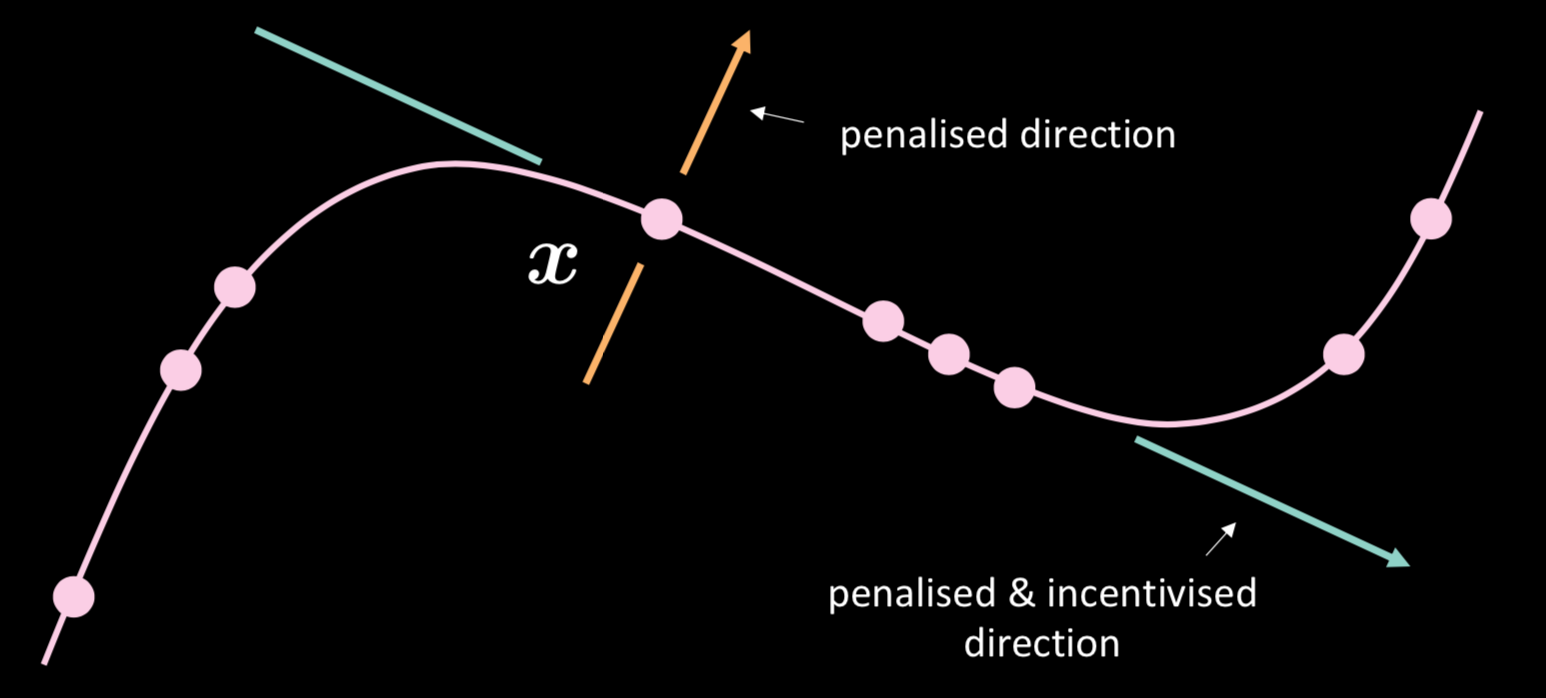
\includegraphics[width=0.6\textwidth]{figs/Contractive_AutoEncoder.png}
    \caption{Illustration of Penalization on Different Directions}
    \label{fig:Contractive_AutoEncoder}
\end{figure}

\subsection{Data Manifold}

Converting data points from data manifold to latent space \textbf{Z} requires knowing the intrinsic dimension of the input. By unwarping the data from higher dimension into lower dimension, we could have data presented in the hidden/latent layer. If we provide start and ending points on the latent space, and calculate the interpolated points between, we could actually interpolate back into higher dimensional space in order to generate other data samples not present in the training data. However, learning this projection from the latent space to the high dimensional space, is challenging. So, often in practice - either learning the distribution of data points or enforcing some structure would be a candidate solution to these shortcomings.

\begin{figure}[htb]
    \centering
    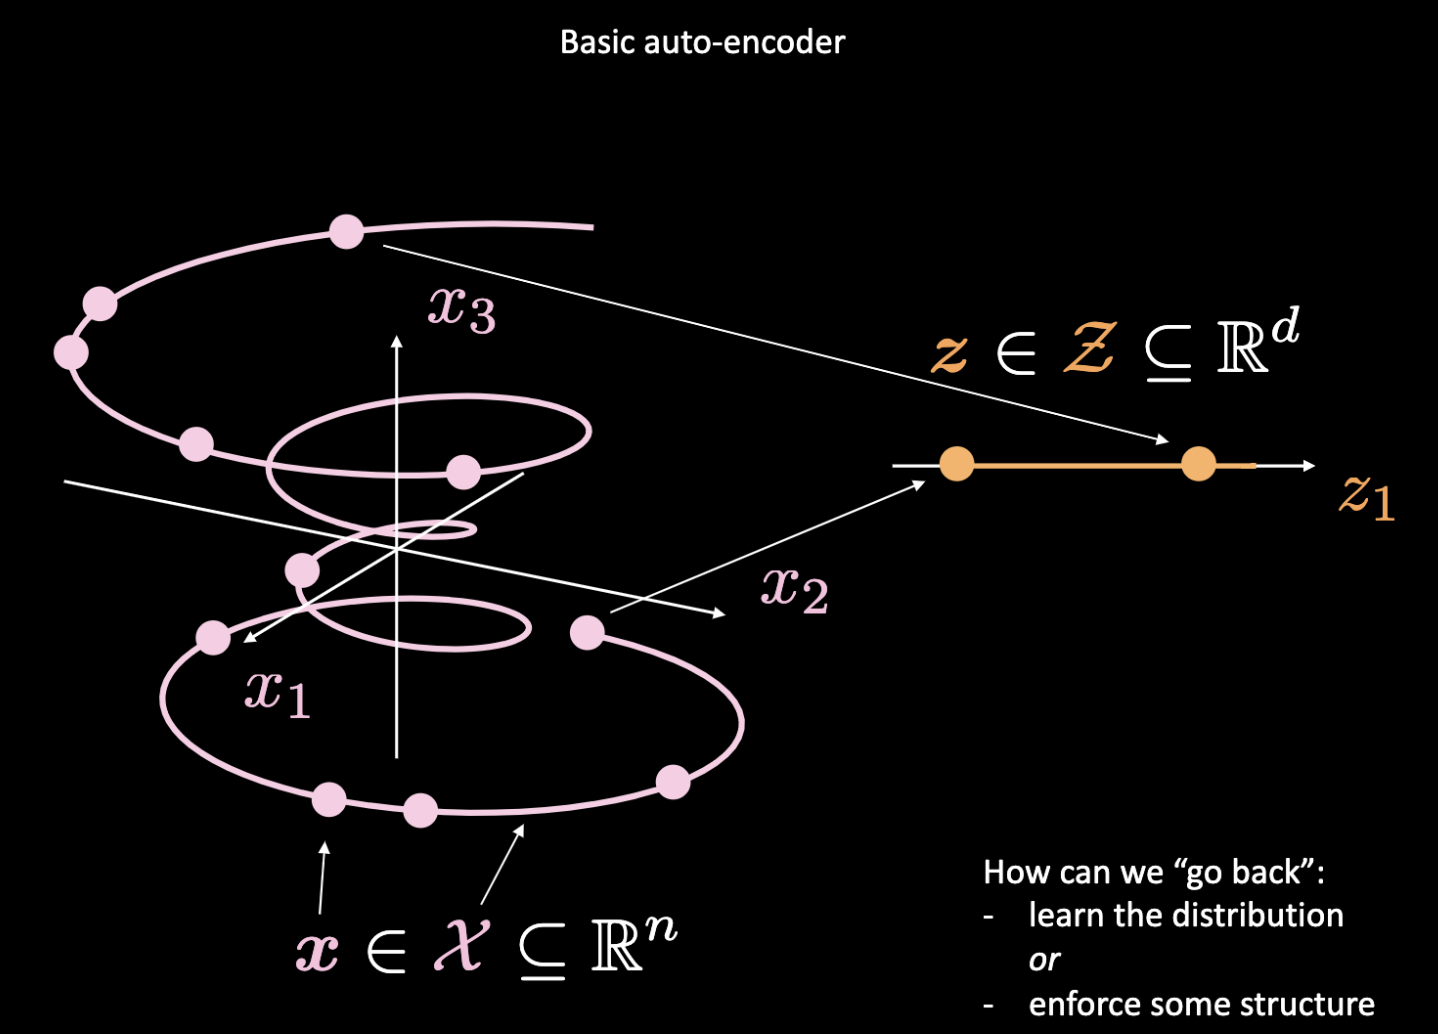
\includegraphics[width=0.6\textwidth]{figs/Data_manifold.png}
    \caption{Illustration on unwarping data manifold}
    \label{fig:Data_manifold}
\end{figure}

\section{Variational Auto-Encoders}
% Authors: Yu Cao, Evgenii Nikitin, Aishwarya Budhkar (editor), 4/16/2019
% Editor: Benjamin Ahlbrand
\begin{figure}[H]
    \centering
    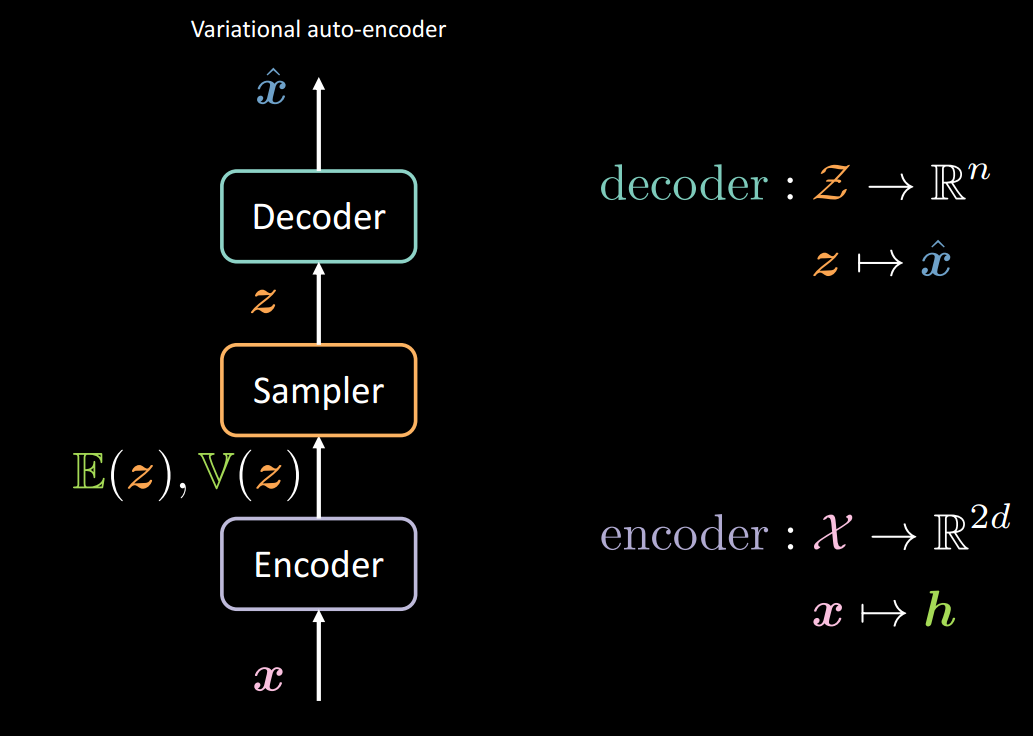
\includegraphics[width=0.7\textwidth]{figs/vae.png}
    \caption{Architecture of Variational Autoencoder}
    \label{fig:vae}
\end{figure}

There are two types of basic autoencoders: over-complete and under-complete. A type of constraint which can be applied is information bottlenecking - this is a reduction in the size of intermediate layer which results in an under-complete autoencoder. In over-complete autoencoders there is larger intermediate layer so we can extract better meaningful features. Variational AutoEncoders (VAE) inherit the architecture of the traditional autoencoders described previously. However, there is a key difference between them -- in contrast to the encoder in a vanilla autoencoder outputting a hidden representation $h$ of the input $x$, the VAE encoder produces two vectors -- expectation $E(z)$ and variance $V(z)$ over latent variable $z$ (Figure \ref{fig:vae}). This property allows us to produce stochastic representations of the input. This is achieved by sampling a vector from a gaussian distribution with zero mean and unit variance and shifting and rescaling vector elements according to estimated $E(z)$ and $V(z)$ respectively:
\begin{align*}
    \vect{z'} &= \mathop{\mathbb{E}}(\vect{z}) + \vect{\epsilon} \odot \sqrt{\mathop{\mathbb{V}}(\vect{z})} \\
    \vect{\epsilon} &\sim \mathcal{N}(0, \mathcal{I}_d)
\end{align*}

After that, sampled representation $z'$ is decoded into output $\hat{x}$. In order to make sure that this output is close to the input $x$, we introduce a reconstruction component of the loss function -- $\ell(x,\hat{x})$ (e.g., mean-squared error loss or binary cross-entropy depending on the nature of the data).

\begin{figure}[H]
    \centering
    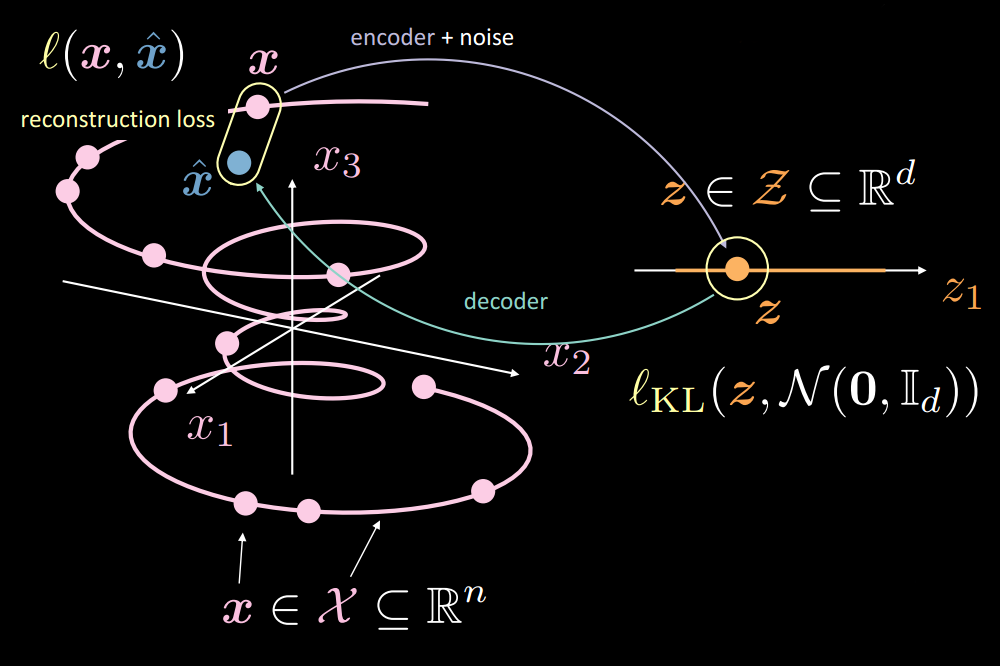
\includegraphics[width=0.7\textwidth]{figs/vae_expl.png}
    \caption{Visualization of encoding and decoding processes}
    \label{fig:vae_expl}
\end{figure}

However, as there is no limit on the values of $E(z)$ and $V(z)$, the encoder can learn to push different training samples very far apart in the latent space (Figure \ref{fig:bubbles_rec}), effectively reconstructing the training data. In order to avoid this, we introduce a constraint by adding KL-divergence component to the loss function.
\begin{align*}
    \ell(x, \hat{x}) = \ell_{rec} + \beta \ell_{KL} (z, \mathcal{N}(0, \mathcal{I}_d)) \simeq \ell_{rec} + \beta\sum_{i=1}^d (\mathop{\mathbb{V}}(\vect{z}) - \log{\mathop{\mathbb{V}}(\vect{z})} - 1 + \mathop{\mathbb{E}}(\vect{z})^2)_i
\end{align*}

Intuitively, this new term forces learned representations of the training samples to have unit variance and to be as close to zero as possible (Figure \ref{fig:bubbles_kl}). $\beta$ is a hyperparameter that controls the tightness of the constraint. Reconstruction loss ensures that the different "bubbles" do not overlap, the network still reconstructs the different inputs, while adding KL-divergence to the reconstruction loss seeks to confine them to the most compact space possible. This feature of VAEs leads to a smooth learned latent spaces, allowing interpolation between the different samples and / or classes continuously.

\begin{figure}[H]
    \centering
    \begin{subfigure}[b]{.45\linewidth}
    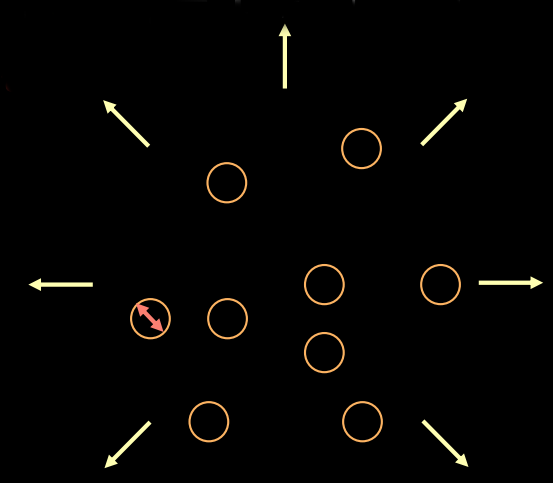
\includegraphics[width=\linewidth]{figs/bubbles_rec.png}
    \caption{Samples get pulled apart by reconstruction loss}\label{fig:bubbles_rec}
    \end{subfigure}
    \begin{subfigure}[b]{.45\linewidth}
    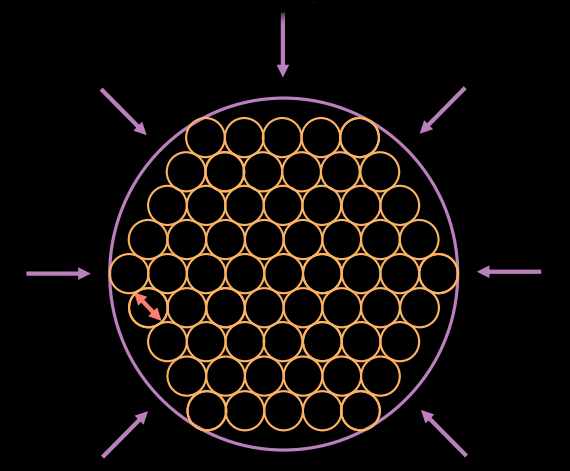
\includegraphics[width=\linewidth]{figs/bubbles_kl.png}
    \caption{Samples get pushed towards zero by KL-divergence loss}\label{fig:bubbles_kl}
    \end{subfigure}
    \caption{Effects of the different loss components}
    \label{fig:bubbles}
\end{figure}

\section{Generative Adversarial Network}
\subsection{Introduction}
\begin{figure}
    \centering
    \includegraphics[width=0.7\textwidth]{"figs/VAE and GAN".png}
    \caption{Architecture of GAN}
    \label{fig:gan_arch}
\end{figure}

As shown in the above figure. The GAN model is conceptually similar to the VAE model.

Consider a money counterfeiter. The $\hat{x}$ produced by sampler+generator can be thought as the fake money he makes. He then tries to deposit the money at a bank (the discriminator), who obviously wants to differentiate fake money from the genuine article ($x$). If the fake money is not 'convincing' enough, the discriminator will provide feedback, stating such, (through back-propagation) and the counterfeiter can improve his skills (gradient descent), until the discriminator can not tell the fake one apart from the genuine one.

Using the sampler we generate noise. On top of the sampler we have the generator which attempts to produce authentic data, similar to the decoder in auto-encoders -- both of which are generative networks. From the generator we get our estimate $\hat{x}$ on the manifold. The estimate, together with our real $x$, is sent to a discriminator which distinguishes $x$ from $\hat{x}$ that is difference between fake and actual values. We can optimize the generator based on what fools and does not fool the discriminator

The generator maps the latent space to input space $\begin{array}{r}{G : \mathcal{Z} \rightarrow \mathbb{R}^{n}}, {z \mapsto \hat{x}}\end{array}$

Whereas the discriminator, we go from the original input ($x$) or the generated input ($\hat{x}$) to a learned loss. $\begin{aligned} D : & \mathbb{R}^{n} \rightarrow(0,1) & x \vee \hat{x} \mapsto \ell \end{aligned}$

\subsection{Model illustration}

\begin{figure}
    \centering
    \includegraphics[width=0.7\textwidth]{"figs/GAN illustration".png}
    \caption{Visualization of encoding and decoding process}
    \label{fig:enc_dec_process}
\end{figure}

We start from a random variable in the hidden space. Then $\hat{x}$ is sampled from the generator. Note that in the GAN setting, we do not know our data manifold, so unlike using reconstruction to approximate $\hat{x}$ to data manifold. We apply our discriminator on both the generated data and real data. We train our discriminator so that it can tell apart the two. On the other hand, we get the gradient, so that we can make the generated data as close to the real data manifold as possible. \\

When training GANs, we don't use a traditional loss function as the scheme here is that of a min-max game. Hence, we instead perform an adversarial loss. See the following equation:

$$V(D, G)=\mathbb{E}_{\boldsymbol{x} \sim p_{\text { data }}(\boldsymbol{x})}[\log D(\boldsymbol{x})]+\mathbb{E}_{\boldsymbol{z} \sim p_{\boldsymbol{z}}(\boldsymbol{z})}[\log (1-D[G(\boldsymbol{z})])]$$
$$\min _{G} \max _{D} V(D, G)$$

The above function achieves a Nash equilibrium between the performance of the discriminator and the performance of the generator. When the two modules converge together, the discriminator should determine fake versus real data, and the generator would generate perfect data.